\documentclass[pdf, aspectratio=169]{beamer}
\usepackage[]{hyperref,graphicx,siunitx,lmodern,booktabs,tikz}
\usepackage{pgfplots,pgfplotstable}
\usepackage[mode=buildnew]{standalone}
\usepackage{intro-commands}
\mode<presentation>{\usetheme{Astro}}

\graphicspath{ {../Images/} }

\sisetup{per-mode=symbol}
\usetikzlibrary{calc,angles,quotes}
\pgfmathdeclarefunction{planck}{1}{\pgfmathparse{1.19E-16/x^5*1/(exp(0.0144/(x*#1))-1)}}

%preamble
\title{Mr Sun, Sun, Mr Golden Sun\ldots}
\date{October 17, 2018}
\author{Jed Rembold}

\begin{document}
\renewcommand*{\theenumi}{\Alph{enumi}}

\begin{frame}{Announcements}
	\begin{itemize}
	  \item WebWork due on Monday
	  \item Test 2 a week from Friday!
		\begin{itemize}
		  \item Chapters 7-14
		  \item I'll post review questions and old tests today if you want to start studying over the long weekend
		  \item Starting today, the new material presented will \alert{not} be on Test 2!
		\end{itemize}
	  \item Polling: \nolinkurl{rembold-class.ddns.net}
	\end{itemize}
\end{frame}

\begin{frame}{APOD}
	\begin{center}
		\begin{tikzpicture}
			\node[nosep](img) at (0,0) {\includegraphics[width=0.6\textwidth]{APOD_Haumea_Ring.jpg}};
			\node[draw,orange,rounded corners, anchor=south west] at (img.south west) {\href{https://apod.nasa.gov/apod/ap171017.html}{Original Link}};
		\end{tikzpicture}
	\end{center}
\end{frame}

\begin{frame}{Review Question!}
  I'm looking into trying to colonize a new planet, and the thing that is most important to me (for whatever reason) is the planet's \emph{size}. Which method of detecting exoplanets would be most useful to me?
  \begin{enumerate}
	\item The astrometric method
	\item The doppler method
	\item \alert<2>{The transit method}
	\item The guess and check method
  \end{enumerate}
\end{frame}

\begin{frame}{Let's talk: The Sun}
  \begin{center}
	\begin{tikzpicture}
	  \node[outer sep=0pt, anchor=center] at (0,0) {\includegraphics[width=7cm]{ch11_sun.jpg}};
	  \node<2->[black, align=right,font=\tiny] at (0,0) {``The sun's rays are the ultimate source of\\almost every motion which takes place on\\the surface of the earth. By its heat are\\produced all winds,\ldots By their vivifying\\action vegetables are elaborated from\\inorganic matter, and become, in their turn,\\the support of animals and of man, and the\\sources of those great deposits of\\dynamical efficiency which are laid up for\\human use in our coal strata''\\ \tiny--John Hershel in his 1833 Treatise on Astronomy};
	\end{tikzpicture}
  \end{center}
\end{frame}

\begin{frame}{A Light Refresher}
  \begin{columns}
	\column{.5\textwidth}
	\begin{itemize}
	  \item There are 3 main attributes of light that we can measure:
		\begin{itemize}
		  \item its direction
		  \item its intensity
		  \item and its wavelength
		\end{itemize}
	\end{itemize}
	\column{.5\textwidth}
	\begin{center}
	  \only<1>{
		\begin{tikzpicture}
		  \node[outer sep=0pt] at (0,0) {\includegraphics[width=.9\textwidth]{ch11_sun_diameter.jpg}};
		  \draw[latex-latex, ultra thick, red] (-2.6,0) -- node[midway,below] {\Large \SI{0.5}{\degree}} (2.6,0);
		\end{tikzpicture}
	  }
	  \includegraphics<2>[width=\textwidth]{ch11_solar-power.jpg}
	  \includegraphics<3>[width=\textwidth]{ch11_sun_spectrum.jpg}
	\end{center}
  \end{columns}
\end{frame}

\begin{frame}{The Light We See}
  \begin{columns}
	\column{.5\textwidth}
	\begin{center}
	  \includegraphics<1>[width=.9\textwidth]{ch11_sun.jpg}
	  \onslide<1>{ The Photosphere}

	  \includegraphics<2>[width=\textwidth]{ch11_corona.jpg}
	  \onslide<2>{ The Corona}
	\end{center}
	\column{.5\textwidth}
	\begin{itemize}
	  \item Almost all the light we see from the sun comes from two places:
		\begin{itemize}
		  \item The surface of the sun (called the photosphere)
		  \item To a much lesser degree, the expansive atmosphere of the sun (called the corona)
		\end{itemize}
	\end{itemize}
  \end{columns}
\end{frame}

\begin{frame}[fragile]{Our Solar Spectrum}
  \begin{center}
	\begin{tikzpicture}
	  \begin{axis}[
		  width=\textwidth,
		  height=7cm,
		  xlabel = Wavelength (\si{\nano\meter}),
		  ylabel = Irradiance (\si{\watt\per\square\meter\per\nano\meter}),
		  xmin = 0,
		  ymin = 0,
		  ticklabel style = {font=\scriptsize},
		  unbounded coords=jump,
		]
		\addplot [mark=none,thick, orange] table[col sep=comma, x index=1, y index=2] {../Data/solar_spectrum.csv};
		\only<2->{
		  \addplot[mark=none, thick, cyan, domain=200e-9:2400e-9, x filter/.code={\pgfmathparse{##1*1e9}\pgfmathresult}, smooth] {planck(5800)/(1.2e13)};
		  \node[cyan,font=\footnotesize,right, align=left] at (axis cs:1200,2) {Wein's Law gives a\\ temperature of 5800 K};
		}
		\only<3>{
		  \node[red!70, font=\footnotesize, right, align=left] at (axis cs:1200,1.3) {Spectrum peaks and lots\\of chemistry gives a mass\\composition of 70\% H,\\28\% He and 2\% other};
		}
	  \end{axis}
	\end{tikzpicture}
  \end{center}
\end{frame}

\begin{frame}{A Distant Tale}
  \begin{itemize}
	\item In order to utilize the light we receive to determine properties of the Sun itself, it is imperative to know how far away the Sun is!
	\item Several different techniques:
	  \begin{itemize}
		\item Initially: parallax
		\item Modern method: radar
		\item Most accurate means find the distance to the planets and then use that to find the distance to the Sun
	  \end{itemize}
  \end{itemize}
  \begin{center}
	\begin{tikzpicture}
	  \node (earth) at (0,0) {\includegraphics[width=5mm]{world.png}};
	  \node[circle, inner color=yellow, outer color=orange, minimum width=1cm] (sun) at (8,0) {};
	  \draw[help lines] (8,0) circle (2cm);
	  \node[circle, fill=red!40, inner sep=0pt, minimum size=3mm] (merc) at ($(8,0)+(104:2cm)$) {};
	  \draw[cyan,dashed] (earth) -- node[midway,above,sloped] {$a\cos(\theta)$} (merc);
	  \draw[cyan,dashed] (merc) -- (sun);
	  \draw[orange,dashed] (earth) -- node[midway,below] {a} (sun);
	  \draw[cyan,<->] (1.5,0) arc (0:14:1.5) node[midway,right,font=\scriptsize] {$\theta$};
	  \draw[cyan] ($(merc)-(14:.3)$) --++(284:.3) --++(14:.3);
	\end{tikzpicture}
  \end{center}
\end{frame}

\begin{frame}{Parallax}
  \begin{itemize}
	\item Parallax is using the idea that looking at the same objects from different vantage points will shift that object's apparent position relative to background objects.
	\item Basic Example: Holding your finger out at arms length and alternating which eye you have open
	\item The \alert{angle} of that shift can be measured
	\item The further away the object, the smaller the effect
	\item The more widely spaced the vantage points, the larger the effect
  \end{itemize}
  \begin{center}
	\begin{tikzpicture}
	  \node[outer sep=0pt, inner sep=0pt] (earth) at (0,0) {\includegraphics[width=5mm]{world.png}};
	  \draw[dashed] (earth) -- +(7,0) node (bg) {$\star$};
	  \draw[help lines] (bg) arc (0:10:7cm) node[outer sep=2pt] {\textcolor{cyan!80}{$\star$}};
	  \draw[help lines] (bg) arc (0:-10:7cm) node[outer sep=2pt] {\textcolor{orange}{$\star$}};

	  \onslide<1>{
		\node[circle, inner sep=0pt, minimum size = 2mm, fill=red!40] (planet) at (3,0) {};
		\draw[shorten >=-4cm, green] (earth.north) -- (planet);
		\draw[shorten >=-4cm, green] (earth.south) -- (planet);
	  }
	  \onslide<2>{
		\node[circle, inner sep=0pt, minimum size = 2mm, fill=red!40] (planet) at (1.5,0) {};
		\draw[shorten >=-6cm, yellow] (earth.north) -- (planet);
		\draw[shorten >=-6cm, yellow] (earth.south) -- (planet);
	  }
	\end{tikzpicture}
  \end{center}
\end{frame}

\begin{frame}{So how far is it?}
  \begin{columns}
	\column{.5\textwidth}
	\begin{itemize}
	  \item Parallax of Mars first measured in 1672
		\begin{itemize}
		  \item Used Paris and French Guyana as the two observation points
		  \item Sun's distance was estimated to approximately 10\% of currently accepted value
		  \item Not bad, but not great either
		\end{itemize}
	\end{itemize}
	\column{.5\textwidth}
	\begin{center}
	  \includegraphics[width=\textwidth]{ch11_mars_parallax.jpg}
	\end{center}
  \end{columns}
\end{frame}

\begin{frame}{Observations of a Lifetime}
  \begin{itemize}
	\item Edmund Halley (of comet fame) predicted that transits of Venus in front of the Sun could be used to calculate Venus's parallax very precisely
	\item He was going to be dead by the time of the next 8 year transit cycle (1761 and 1769), so he laid out very careful instructions
	\item Theory is easier than reality
	  \begin{itemize}
		\item Astronomer had to know their location on Earth very precisely
		\item Areas where the transit would be visible were in remote parts of the Earth
		\item Most astronomers were English or French, who were in the middle of the 7 years war
		\item Wild stories including:
		  \begin{itemize}
			\item Warding off superstitious peasants
			\item Drinking away harsh winters
			\item Surviving multiple attacks by ship
			\item Keeping sailors from trading the very nails in your ship for ``favors'' from Taihitan women
			\item More stories \href{http://www.astronomy.ohio-state.edu/~pogge/Ast161/Unit4/venussun.html}{\textcolor{LOrange}{here}}
		  \end{itemize}
	  \end{itemize}
  \end{itemize}
\end{frame}

\begin{frame}{Success!}
  \begin{columns}
	\column{.5\textwidth}
	\begin{itemize}
	  \item In the end, the mission was successful!
	  \item Calculated the distance to the Sun within 2\% of the established value
	  \item Discovered the ``Black Drop'' effect, caused by Earth's atmosphere
	  \item Today the value of 1 AU is known within \alert{\SI{30}{\meter}}!
	\end{itemize}
	\column{.5\textwidth}
	\begin{center}
	  \begin{tikzpicture}
		\clip[rounded corners] (.3,.2) rectangle (4.9,4.9);
		\node[anchor=south west, outer sep=0pt] at (0,0) {\includegraphics[width=5cm]{ch11_venus_transit.png}};
	  \end{tikzpicture}
	\end{center}
  \end{columns}
\end{frame}

\begin{frame}{Understanding Check}
  Suppose we see some distant (orange) object from the Earth, and measure its angular distance from the star Antares at different points of the year. When will we see the object as being closest to Antares?
  \begin{center}
	\begin{tikzpicture}
	  \draw[dashed] (0,0) circle (1cm);
	  \fill[inner color=yellow, outer color=orange] (0,0) circle (3mm);
	  \node[inner sep=0pt, outer sep=0pt] (earth) at (45:1) {\includegraphics[width=2mm]{world.png}};
	  \node[ball color=orange, circle, minimum size=6pt, inner sep=1pt] (p) at (7,0) {};
	  \draw[help lines] (-10:8) arc (-10:10:8);
	  \node[yellow, label={right:Antares}] at (10:8) {\LARGE$\star$};

	  \node[cyan] (A) at (0:1.2) {A};
	  \node[cyan] (B) at (90:1.2) {B};
	  \node[cyan] (C) at (180:1.2) {C};
	  \node[cyan] (D) at (270:1.2) {D};

	  \pause
	  \draw<+->[red, dashed, shorten >=-1cm] (A) -- (p);
	  \draw<+->[red, dashed, shorten >=-1cm] (B) -- (p);
	  \draw<+->[red, dashed, shorten >=-1cm] (C) -- (p);
	  \draw<+->[green, shorten >=-1cm] (D) -- (p);
	\end{tikzpicture}
  \end{center}
\end{frame}

\begin{frame}{The Pieces Fall Together}
  \begin{itemize}
	\item Once we have a handle on the distance, we can determine:
	  \begin{itemize}
		\item The Radius of the Sun ($\approx \SI{700000}{\kilo\meter}$)
		  \begin{itemize}
			\item From the angular size and distance
		  \end{itemize}
		\item The Luminosity of the Sun ($\approx \SI{4E26}{\watt}$)
		  \begin{itemize}
			\item From the apparent brightness and distance
		  \end{itemize}
		\item The Mass of the Sun ($\approx \SI{2e30}{\kilo\gram}$)
		  \begin{itemize}
			\item From Kepler, Newton, and the Earth's orbit
		  \end{itemize}
	  \end{itemize}
  \end{itemize}
  \begin{center}
	\includegraphics[width=.5\textwidth]{ch11_mercury_transit.jpg}
  \end{center}
\end{frame}

\begin{frame}{Aren't You Bright!}
  \begin{itemize}
	\item The \underline{luminosity} of the Sun is the total power output of the Sun, measured in watts (eg. joules per second)
	\item You can estimate it two different ways:
  \end{itemize}
  \begin{columns}[t]
	\column{.5\textwidth}
	\begin{block}{Brightness from Earth}
	  \scriptsize
	  \begin{align*}
		L &= 4\pi d^2 \times B \\
		&= 4\pi\left( \SI{1.5e11}{\meter} \right)^2 \times \left( \SI{1400}{\watt\per\square\meter} \right) \\
		&\approx \SI{4e26}{\watt}
	  \end{align*}
	  where $B$ is the brightness we see at Earth and $d$ is the distance to the Sun
	\end{block}
	\column{.5\textwidth}
	\begin{block}{Size and Temperature}
	  \scriptsize
	  \begin{align*}
		L &= 4\pi R^2 \times I \\
		&= 4\pi R^2 \times (\sigma T^4) \\
		&= 4\pi \left( \SI{7e8}{\meter} \right)^2\\
		&\quad\times \left( \SI{5.7E-8}{\watt\per\square\meter\per\kelvin^4} \left( \SI{5800}{\kelvin} \right)^4 \right)\\
		&\approx \SI{4e26}{\watt}
	  \end{align*}
	  where $R$ is the radius of the Sun, $T$ is the temperature of the Sun, and $\sigma$ is the Stefan-Boltzmann constant.
	\end{block}
  \end{columns}
\end{frame}

\begin{frame}{Confusion!}
  \begin{itemize}
	\item Be careful not to confuse the \alert{luminosity} with the \alert{intensity} of the Sun!
	\item Intensity is the same as Brightness, and is a measure of how much energy hits an \alert{area} in a certain amount of time
	\item Luminosity is a measure of how much energy is spewed out of an object (regardless of size) in an amount of time
  \end{itemize}
  \begin{alertblock}{Rule of Thumb:}
	When in doubt, let the units guide you. \si{\watt\per\meter^2} is a brightness or intensity, while just \si{\watt} is a luminosity!
  \end{alertblock}
\end{frame}

\begin{frame}{Asking the Key Questions\ldots}
  \begin{itemize}
	\item Now that we understand the physical parameters of the Sun, we can attempt to answer some questions about it
	\item Most obviously:
  \end{itemize}
  \begin{center}
	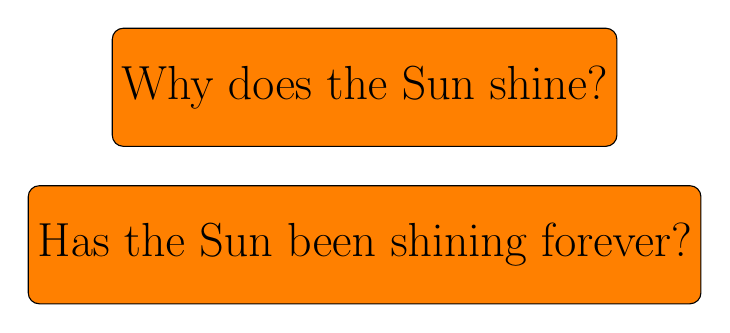
\begin{tikzpicture}
	  \node[rounded corners, minimum width=5cm, minimum height=1.5cm, fill=orange, draw=black, text=black, font=\LARGE] at (0,0) {Why does the Sun shine?};
	  \node[rounded corners, minimum width=5cm, minimum height=1.5cm, fill=orange, draw=black, text=black, font=\LARGE] at (0,-2) {Has the Sun been shining forever?};
	\end{tikzpicture}
  \end{center}
\end{frame}

\begin{frame}{Why so shiny?}
  \begin{itemize}
	\item Shining means the Sun is giving off energy
	\item Where it gets this energy was a major question of the early 1900s
	  \begin{itemize}
		\item Originally thought to be some sort of chemical burning
		  \begin{itemize}
			\item First estimates of the luminosity demanded WAY too much energy
			\item Would only have enough fuel for 16000 years
		  \end{itemize}
		\item Gravitational Contraction?
		  \begin{itemize}
			\item Could burn for 25 million years\ldots
			\item But Earth's fossil record indicates Earth is older than that?
		  \end{itemize}
	  \end{itemize}
  \end{itemize}
  \begin{center}
	\includegraphics[width=.3\textwidth]{ch11_shining_sun.png}
  \end{center}
\end{frame}

%\begin{frame}{Stability}
  %\begin{itemize}
	%\item Regardless of energy source, why doesn't the Sun use up all it's fuel at once?
	%\item If you light a match, it flares up and then burns out. No steady glow.
	%\item Defying Gravity:
	  %\begin{itemize}
		%\item Gravity pulling everything inward
		%\item Sun has not collapsed into a tiny ball over all these years
		%\item Therefore, something must be working against gravity!
		  %\begin{itemize}
			%\item \alert{Gas Pressure}
		  %\end{itemize}
	  %\end{itemize}
  %\end{itemize}
%\end{frame}

%\begin{frame}{Under Pressure \scriptsize (dum dum dum bada dumdum)}
  %\begin{itemize}
	%\item We know molecules speed up when they get hot
	%\item Pressure is a measure of how hard those molecules hit the edges of their container
	%\item Hotter = Faster = More Energy = Harder Hitting
	%\item So pressure and temperature are linked! (Almong other things. Ideal Gas Law)
	%\item As the Sun contracts, the warming molecules will push back with more force
	%\item At some point, a balance is reached!
  %\end{itemize}
  %\begin{center}
	%\begin{tikzpicture}[scale=1]
	  %\shade[left color = orange, right color=yellow] (0,0) --++(4,0) arc (-10:10:8cm) --++(-4,0) -- cycle;
	  %%\draw[ultra thick, orange] (4,0) arc (0:10:8cm);
	  %%\draw[ultra thick, orange] (4,0) arc (0:-10:8cm);
	  %\foreach \p in {1,2,...,20}{
		%\fill[ball color=red] (rnd*4,rnd*2.6+.1) coordinate (p) circle (2pt);
		%\draw[-latex, black] (p) --+(rnd*360:3mm);
	  %}
	  %\draw[ultra thick, cyan, -latex] (4,3) --+(-1,0) node[left] {$F_{gravity}$};
	  %\draw[ultra thick, red, -latex] (4,3) --+(1,0) node[right] {$F_{pressure}$};
	%\end{tikzpicture}
  %\end{center}
%\end{frame}

%\begin{frame}{Gotta stay Balanced}
  %\begin{columns}
	%\column{.5\textwidth}
	  %\begin{itemize}
		%\item Everywhere in the star needs to be balanced
		%\item The weight the pressure needs to support increases as we go deeper
		%\item Pressure must therefore increase
		%\item And thus temperature and density must also increase
	  %\end{itemize}
	%\column{.5\textwidth}
	%\begin{center}
	  %\begin{tikzpicture}[scale=.9, transform shape]
		%\clip[rounded corners] (.1,.1) rectangle (4.5,7);
		%\node[inner sep=0pt, outer sep=0pt, anchor=south west] at (0,0) {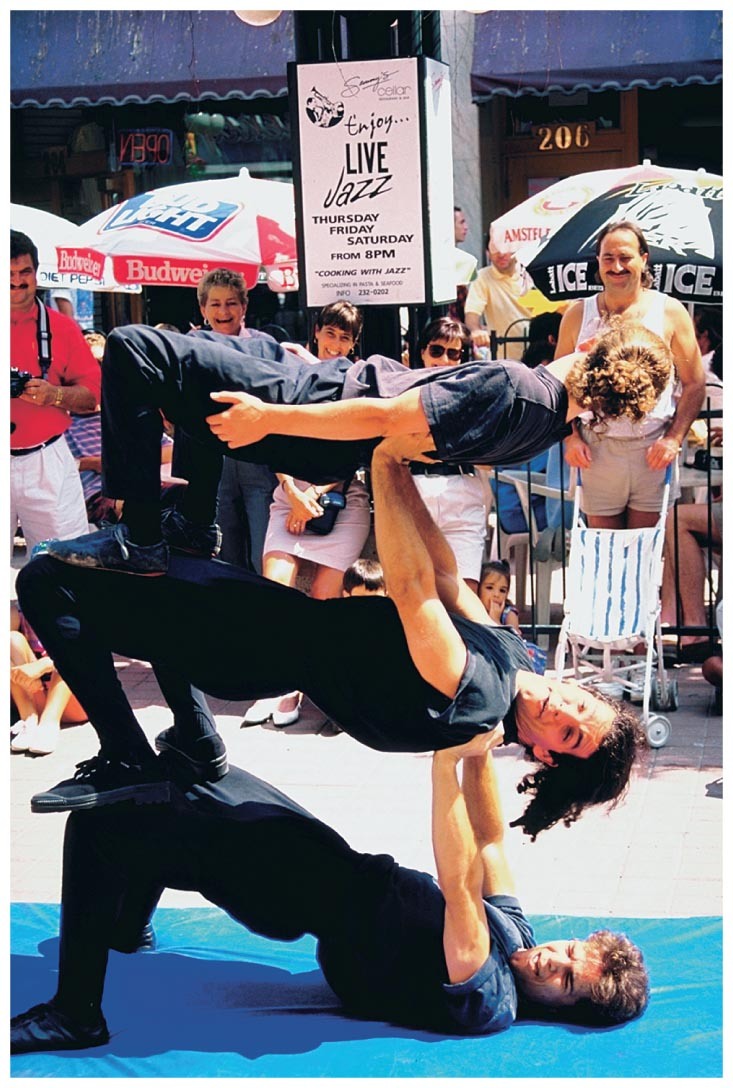
\includegraphics[width=.7\textwidth]{ch11_human_stack.jpg}};
	  %\end{tikzpicture}
	%\end{center}
  %\end{columns}
%\end{frame}

\end{document}
